%قبل از شروع مسئله ترجیحاً چیزی ننویسید. اما اگر خواستید بنویسید، در قالب لیستی (فقرات و شمارش) بنویسید.
\شروع‌مسئله[10] \متن‌سیاه{سؤال‌های جواب کوتاه.}
% صورت اصلی مسئله را در این‌جا بنویسید.
\شروع{زیرمسائل}
\زیرمسئله[5]
چرا الگوریتم مرتب‌سازی سریع در زبان برنامه‌نویسی سی‌پلاس‌پلاس و جاوا (برای مرتب کردن اعداد) به جای مرتب‌سازی ادغامی استفاده می‌شود. حداقل ۲ دلیل ذکر کنید.


\پاسخ{
\begin{enumerate}
	\item تقریبا ۲ برابر سریع‌تر است.
	\item 
	حافظه اضافی زیادی نمی‌خواهد.
\end{enumerate}
}
\زیرمسئله[5]
یک درخت قرمز-سیاه مثال بزنید که AVL نباشد.

\پاسخ{
درختان زیادی وجود دارد. به عنوان مثال:
\begin{center}
	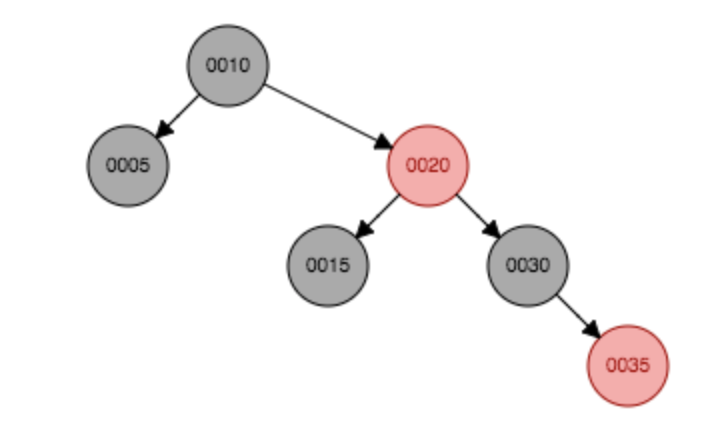
\includegraphics[width=0.5\columnwidth]{RBT.png}
\end{center}
}
%\زیرمسئله[4]
%این جمله درست است یا غلط؟ اگر عنصری با کلید $a$ در یک درخت AVL برگ نباشد، عنصر با کوچک‌ترین  کلید بزرگ‌تر از $a$ حتماً برگ است.

\پایان{زیرمسائل}